\section*{13 : Proyectos}
\label{sec:proy}
\addcontentsline{toc}{section}{\nameref{sec:proy}}

Una serie de proyectos más desafiantes para que usted pueda resolver. \newline

[[Algunos de estos pueden convertirse en ejemplos en el libro, por lo que en algún momento podría desaparecer de aquí]]


\subsection*{Ratas y Laberintos}
\label{subsec:ratas}
\addcontentsline{toc}{subsection}{\nameref{subsec:ratas}}

Primero, crea un \textit{Blackboard }\newline(citar esta referencia) que es un objeto sobre el que cualquier persona puede registrar la información. Este Blackboard particular  dibuja un laberinto, y es usado como información que vuelve sobre la estructura de un laberinto desde  las ratas que lo están  buscando. \newline

Ahora cree el propio laberinto. Como un laberinto real, este objeto revela muy poca información sobre si mismo \-dada una coordenada, que le dirá si hay paredes o espacios en las cuatro direcciones  inmediatamente que coordinan, pero no más.  Para empezar, lea el laberinto desde un archivo de texto pero considere la busqueda en internet para un algoritmo que genere un laberinto. En cualquier caso, el resultado debe ser un objeto que, dado una coordenada del laberinto, informará paredes y espacios alrededor de esa coordenada. Además, debe ser capaz de preguntar por un punto de entrada al laberinto.  \newline

Finalmente, crear la clase \textbf{Rat} laberinto-buscar. Cada rata puede comunicarse tanto con el Blackboard para dar la información actual y el laberinto para solicitar neva información sobre la base de la posición actual de la rata. Sin embargo, cada vez que una rata llega a un punto de decisión donde se ramifica el laberinto, crea una nueva rata que baja por cada una de las ramas. Cada rata es conducida por su propio hilo. Cuando una rata llega a un callejón sin salida, termina en sí después de informar los resultados de su búsqueda final al Blackboard.\newline

El objetivo es trazar un mapa completo del laberinto, pero también usted debe determinar si la condición final será encontrada naturalmente o si el blackboard debe ser responsable de la decisión. \newline

Un ejemplo de implementación de Jeremy Meyer:    \newline

\begin{lstlisting}
# c13:Maze.py 

class Maze(Canvas): 
  private Vector lines # a line is a char array 
  private int width = -1 
  private int height = -1 
  public static void main (String [] args)  
  throws IOException: 
    if (args.length < 1): 
      print ``Enter filename" 
      System.exit(0) 
      
    Maze m = Maze() 
    m.load(args[0]) 
    Frame f = Frame() 
    f.setSize(m.width*20, m.height*20) 
    f.add(m)      
    Rat r = Rat(m, 0, 0) 
    f.setVisible(1) 
    
  def __init__(self): 
    lines = Vector() 
    setBackground(Color.lightGray) 
    
  synchronized public boolean  
  isEmptyXY(int x, int y): 
    if (x < 0) x += width 
    if (y < 0) y += height  
    # Use mod arithmetic to bring rat in line: 
    byte[] by =  
      (byte[])(lines.elementAt(y%height))   
    return by[x%width]==' ' 
    
  synchronized public void  
  setXY(int x, int y, byte newByte): 
    if (x < 0) x += width 
    if (y < 0) y += height  
    byte[] by =  
      (byte[])(lines.elementAt(y%height)) 
    by[x%width] = newByte 
    repaint() 
    
  public void  
  load(String filename) throws IOException: 
    String currentLine = null 
    BufferedReader br = BufferedReader( 
      FileReader(filename)) 
    for(currentLine = br.readLine()  
        currentLine != null 
        currentLine = br.readLine()) : 
      lines.addElement(currentLine.getBytes())        
      if(width < 0 ||  
         currentLine.getBytes().length > width) 
        width = currentLine.getBytes().length 
        
    height = len(lines) 
    br.close() 
    
  def update(self, Graphics g): paint(g)  
  public void paint (Graphics g): 
    int canvasHeight = self.getBounds().height 
    int canvasWidth  = self.getBounds().width 
    if (height < 1 || width < 1)  
      return # nothing to do  
    int width =  
      ((byte[])(lines.elementAt(0))).length 
    for (int y = 0 y < len(lines) y++): 
      byte[] b 
      b = (byte[])(lines.elementAt(y)) 
      for (int x = 0 x < width x++): 
        switch(b[x]): 
          case ' ': # empty part of maze 
            g.setColor(Color.lightGray) 
            g.fillRect( 
              x*(canvasWidth/width), 
              y*(canvasHeight/height), 
              canvasWidth/width, 
              canvasHeight/height) 
            break 
          case '*':     # a wall  
            g.setColor(Color.darkGray) 
            g.fillRect( 
              x*(canvasWidth/width), 
              y*(canvasHeight/height), 
              (canvasWidth/width)-1, 
              (canvasHeight/height)-1) 
            break 
          default:      # must be rat 
            g.setColor(Color.red) 
            g.fillOval(x*(canvasWidth/width), 
            y*(canvasHeight/height), 
            canvasWidth/width, 
            canvasHeight/height) 
            break              
            
# :~ 

# c13:Rat.py 

class Rat: 
  static int ratCount = 0 
  private Maze prison 
  private int vertDir = 0  
  private int horizDir = 0 
  private int x,y 
  private int myRatNo = 0 
  def __init__(self, Maze maze, int xStart, int 
yStart): 
    myRatNo = ratCount++ 
    print ("Rat no." + myRatNo +  
      " ready to scurry.") 
    prison = maze 
    x = xStart 
    y = yStart 
    prison.setXY(x,y, (byte)'R') 
    Thread(): 
      def run(self){ scurry()  
    .start() 
    
  def scurry(self): 
    # Try and maintain direction if possible. 
    # Horizontal backward 
    boolean ratCanMove = 1 
    while(ratCanMove): 
      ratCanMove = 0 
      
      # South  
      if (prison.isEmptyXY(x, y + 1)): 
        vertDir = 1 horizDir = 0          
        ratCanMove = 1
        
      # North 
      if (prison.isEmptyXY(x, y - 1)) 
        if (ratCanMove) 
          Rat(prison, x, y-1) 
          # Rat can move already, so give  
          # this choice to the next rat. 
        else: 
          vertDir = -1 horizDir = 0          
          ratCanMove = 1 
          
      # West 
      if (prison.isEmptyXY(x-1, y)) 
        if (ratCanMove) 
          Rat(prison, x-1, y)    
          # Rat can move already, so give  
          # this choice to the next rat. 
        else: 
          vertDir = 0 horizDir = -1          
          ratCanMove = 1 
          
      # East 
      if (prison.isEmptyXY(x+1, y)) 
        if (ratCanMove) 
          Rat(prison, x+1, y)    
          # Rat can move already, so give  
          # this choice to the next rat. 
        else: 
          vertDir = 0 horizDir = 1          
          ratCanMove = 1 
          
      if (ratCanMove): # Move original rat. 
        x += horizDir 
        y += vertDir 
        prison.setXY(x,y,(byte)'R') 
        # If not then the rat will die. 
      try: 
        Thread.sleep(2000)    
       catch(InterruptedException ie): 
       
    print ("Rat no." + myRatNo +  
      " can't move..dying..aarrgggh.") 
      
# :~     
    
\end{lstlisting}

El archivo de inicialización de laberinto:

%% AGREGAndo IMAGEN
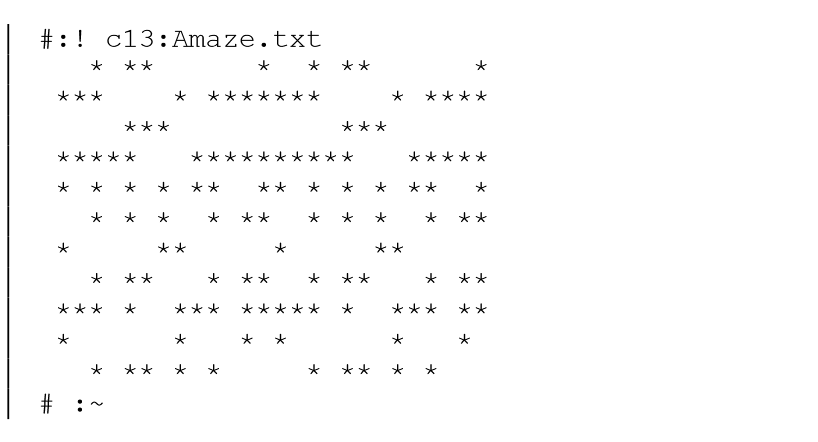
\includegraphics[width=\textwidth]{ultimaimagenTIP}


\subsubsection*{Otros Recursos para Laberinto}
\label{subsubsec:orpl}
\addcontentsline{toc}{subsubsection}{\nameref{subsubsec:orpl}}


Una discusión de algoritmos para crear laberintos así como el código fuente de Java para implementarlas : \newline

\textcolor[rgb]{0.2,0.5,0.7}{\underline{http://www.mazeworks.com/mazegen/mazegen.htm}} \newline      % COLOR AZUL

Una discusión de algoritmos para la detección de colisiones y otros comportamientos de movimiento individual/grupal de los objetos físicos autónomos: \newline

\textcolor[rgb]{0.2,0.5,0.7}{\underline{http://www.red3d.com/cwr/steer/}}


\subsubsection*{Decorador XML}
\label{subsubsec:dxml}
\addcontentsline{toc}{subsubsection}{\nameref{subsubsec:dxml}}


Crear un par de decoradores para I/O Los lectores y escritores que codifican (para el decorador Escritor) y decodificación XML.